Uživatel má několik možností, jak získat model \smod. 
% Pomocí instalačního souboru lze nainstalovat \smod jako běžný Python balíček. 
Model \smod je poskytován ve formě zdrojového kódu. Je tedy možné spouštět 
balíček přímo bez instalace. V této části manuálu je popsáno jak získat mode \smod a jak ho použít
v prostředí ArcGIS.
  
Model \smod je distribuován pod GPLv3\footnote{Více informací na: 
\href{https://www.gnu.org/licenses/gpl-3.0.en.html}{gnu.org/licenses/gpl-3.0.en.html}} licencí. 
Veškeré dostupné  materiály lze stáhnout na webových stránkách Katedry hydromeliorací 
a krajinného inženýrství, Fakulty stavební ČVUT 
v Praze~(\href{http://storm.fsv.cvut.cz/cinnost-katedry/volne-stazitelne-vysledky/smoderp/}{storm.fsv.cvut/../smoderp/}). 
Na odkazu lze stáhnout malíček modelu \smod, tento manuál a další aktuální informace včetně odkazu na vzdálený 
repozitář na platformě {\tt github.com}, kde je vždy dostupná aktuální verze modelu. 



% Instalační soubor pro operační systém Windows lze stáhnout na adrese~\href{http://storm.fsv.cvut.cz/cinnost-katedry/volne-stazitelne-vysledky/smoderp/program-smoderp2d/}{storm.fsv.cvut/../smodep/program-smoderp2d/} na odkazu: Instalační EXE soubor pro Windows. Po spuštění souboru se otevře průvodce k instalaci standardního balíčku Python (úvodní obrazovka průvodce je ukázána na obrázku~\ref{fig:pruvodce}). Po ukončení instalace lze model \smod importovat do Python skriptu příkazem {\tt import smoderp2d.main}. 

% Před použitím modelu se doporučuje provést test, který ověří, zda má uživatel nainstalované ostatní používané balíčky. Testovací skript je spolu s testovacími daty ke stažení na adrese ~\href{http://storm.fsv.cvut.cz/cinnost-katedry/volne-stazitelne-vysledky/smoderp/program-smoderp2d/}{storm.fsv.cvut/../smodep/program-smoderp2d/} na odkazu: Test po instalaci. Testovací skript s názvem {\tt importrun.py} uložte do společné složky s testovacími daty {\tt test-data}. Po spuštění skriptu se otevře okno terminálu příkazové řádky. Pokud instalace balíčku \smod neproběhla nebo proběhla chybně, vypíše testovací skript hlášení ukázané na obrázku~\ref{fig:importerror}. Pokud nejsou nainstalované jiné nezbytné balíčky, může se chybové hlášení lišit. Pokud například chybí balíček {\tt numpy}, vypíše se na třetí řádek hlášení: {\tt No module named numpy}. V takovém případě je nutné chybějící balíčky doinstalovat běžným způsobem. Pokud proběhne testovací běh modelu \smod bezchybně, proběhne v okně terminálu hlášení ukázané na obrázku~\ref{fig:testok}. Výstupní soubory jsou pak uložený do složky {\tt test-out} v adresáři kde je uložen skript {\tt importrun.py}. V tento moment je model \smod včetně nezbytných balíčků zdárně nainstalován a je připraven k použití.
  
% \begin{figure}[t!]
%    \centering
%    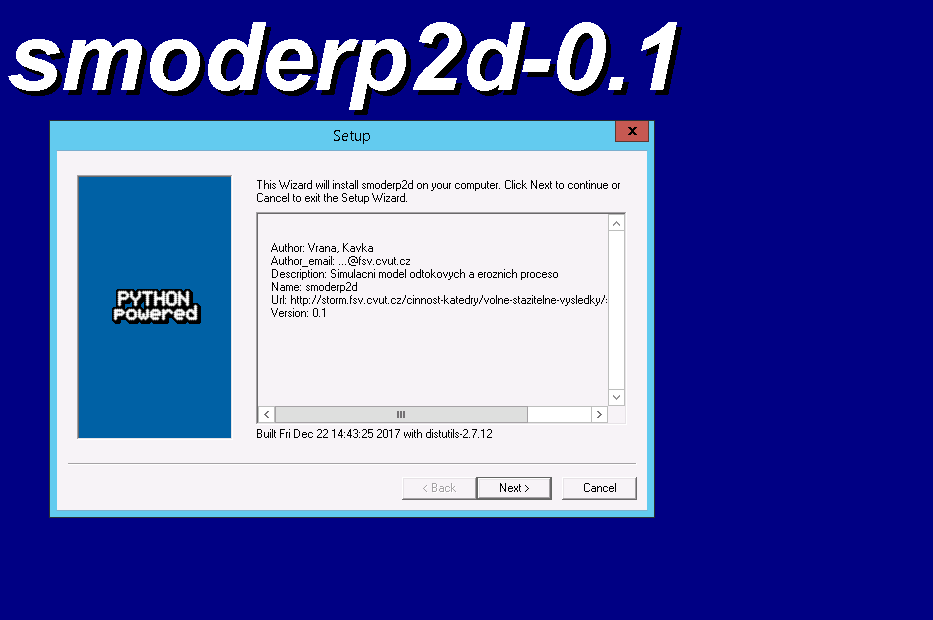
\includegraphics[width=0.75\textwidth]{./img/instalace.png}
%    \caption{Úvodní obrazovka při instalaci balíčku \smod}
%    \label{fig:pruvodce}
%  \end{figure}
% 
%  \begin{figure}[b!]
%    \centering
%    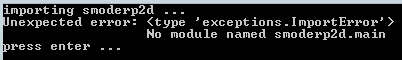
\includegraphics[width=0.75\textwidth]{./img/importerror.png}
%    \caption{Hlášení při chybné instalaci balíčku modelu \smod}
%    \label{fig:importerror}
%  \end{figure}
% 
%  \begin{figure}[t!]
%    \centering
%    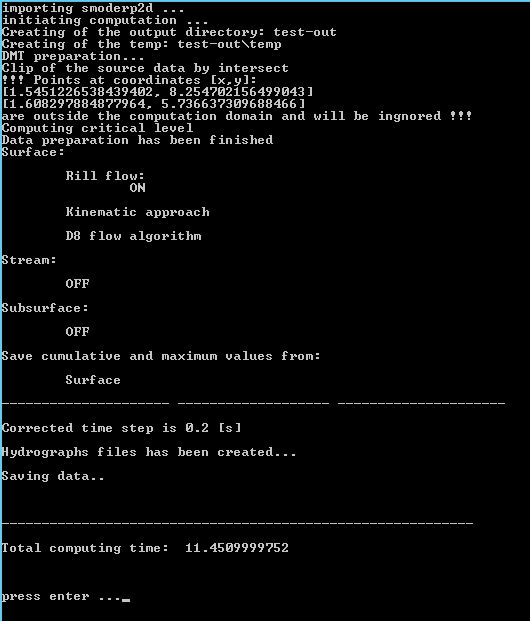
\includegraphics[width=0.75\textwidth]{./img/testok.png}
%    \caption{Zdárný průběh testovacího skriptu modelu}
%    \label{fig:testok}
%  \end{figure}
  
\subsection{Použití modelu v ArcGIS}
  
Současná verze modelu \smod využívá k přípravě vstupních dat výhradně software ArcGIS a Python balíček {\tt arcpy}. 
Proto je součástí staženého modelu ArcGIS toolbox, který umožní, po nalinkování kořenohového adresáře modelu, 
spouštět model \smod přímoz prostředí ArcMAP. Spuštěný nalinkovaný a toolbox je ukázán na obrázku \ref{git:toolboxlink}
Takto připravený toolbox s poskytnutými testovacími daty je možné pustit bez dalších modifikací a následně si prohlédnout 
výsledky modelu (jednotlivé výstupy modelu jsou popsány dále v textu). 

Vysvětlení jednotlivých vstupů v celém toolboxu je ukázáno na obrázku~\ref{fig:toolbox}

% Proto je potřeba vytvořit spouštěcí skript, který načte a spustí model \smod. Takový skript může obsahovat následující příkazy:
% %   \begin{figure}[h!]
%     \begin{lstlisting}
%       import smoderp2d.main as sm
%       sm.run()
%     \end{lstlisting}
% %     \caption{Skript pro spuštění modelu \smod}
% %   \end{figure}
%   {\tt import smoderp2d.main as sm}  načte balíček modelu \smod. Spuštěním metody  {\tt sm.run()} je spuštěn samotný model. 
%   
%   Pro použití modelu v prostředí ArcGIS je třeba vytvořit ArcGIS {\tt toolbox}, kde je nastavený jako zdrojový soubor  uložený spouštěcí skript. Další krok je nastavení parametrů ArcGIS {\tt toolbox} odkud se načítají vstupní parametry do modelu. Pořadí zadávaných hodnot je {\bf nutné dodržet}! Ukázka ArcGIS {\tt toolbox} a vysvětlení parametrů je ukázáno na obrázku~\ref{fig:toolbox}. Připravený ArcGIS {\tt toolbox} a spouštěcí skript lze stáhnout na adrese~\href{http://storm.fsv.cvut.cz/cinnost-katedry/volne-stazitelne-vysledky/smoderp/program-smoderp2d/}{storm.fsv.cvut/../smodep/program-smoderp2d/} na odkazu: Použití modelu v ArcGIS. Detailnější popis vstupních hodnot je v kapitole~\ref{kap:vstupy}.
  
 \begin{figure}[t!]
    \centering
    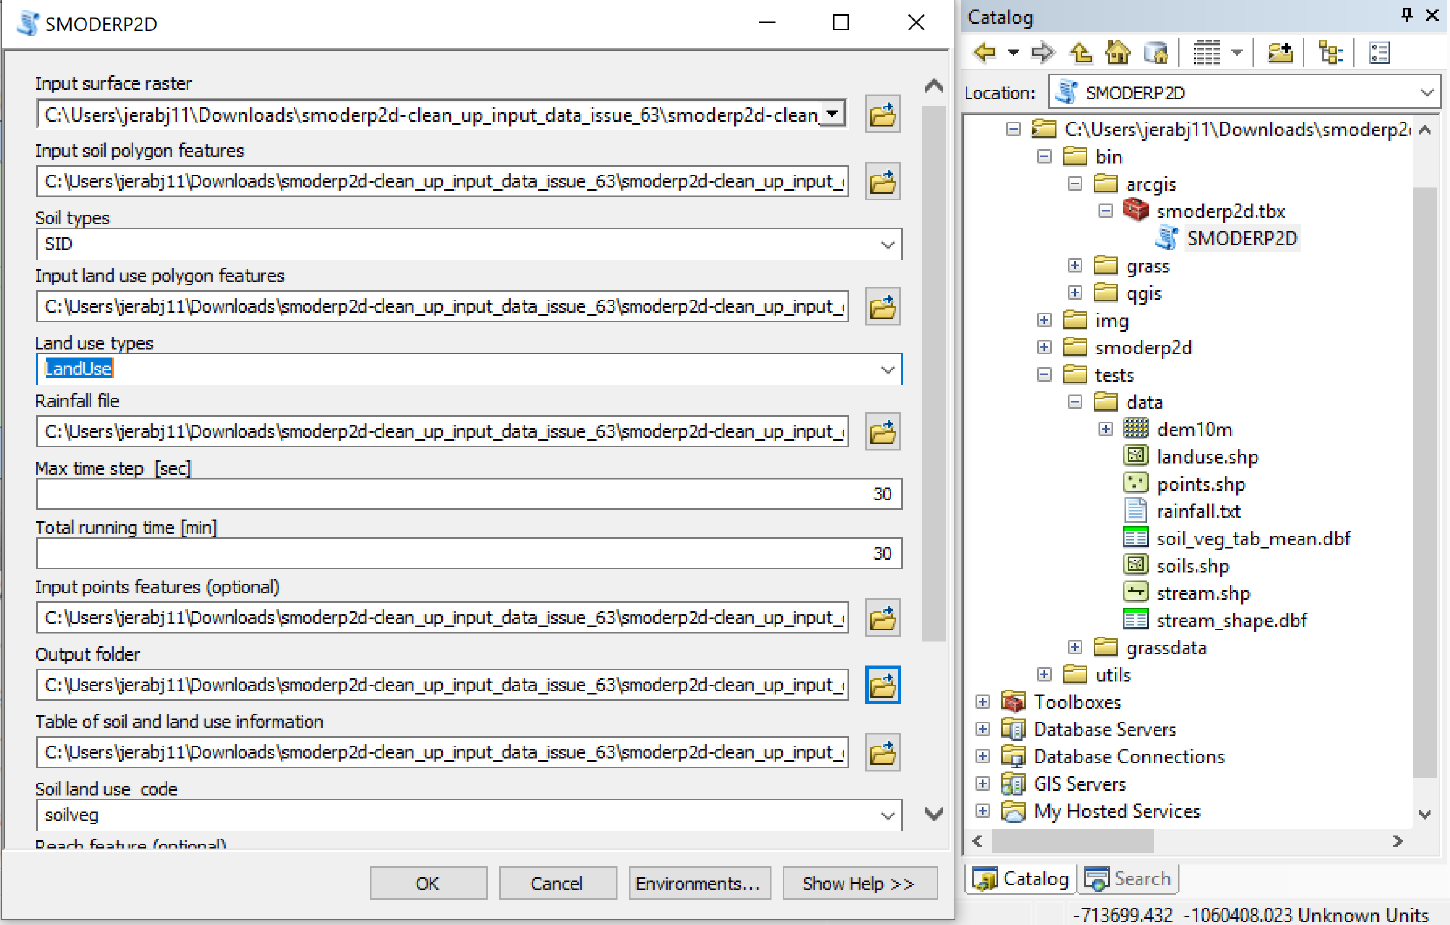
\includegraphics[width=1.0\textwidth]{./img/arcmap01.png}
     \caption{Nalinkovaný smoderpěd ArcGIS toolbox do prostředí ArcMAP pomocí Arc Catalogu}
    \label{fig:toolboxlink}
  \end{figure}

  
  \begin{figure}[t!]
    \centering
    \begin{minipage}[t]{.45\textwidth}
      \centering
      \vspace{0pt}
      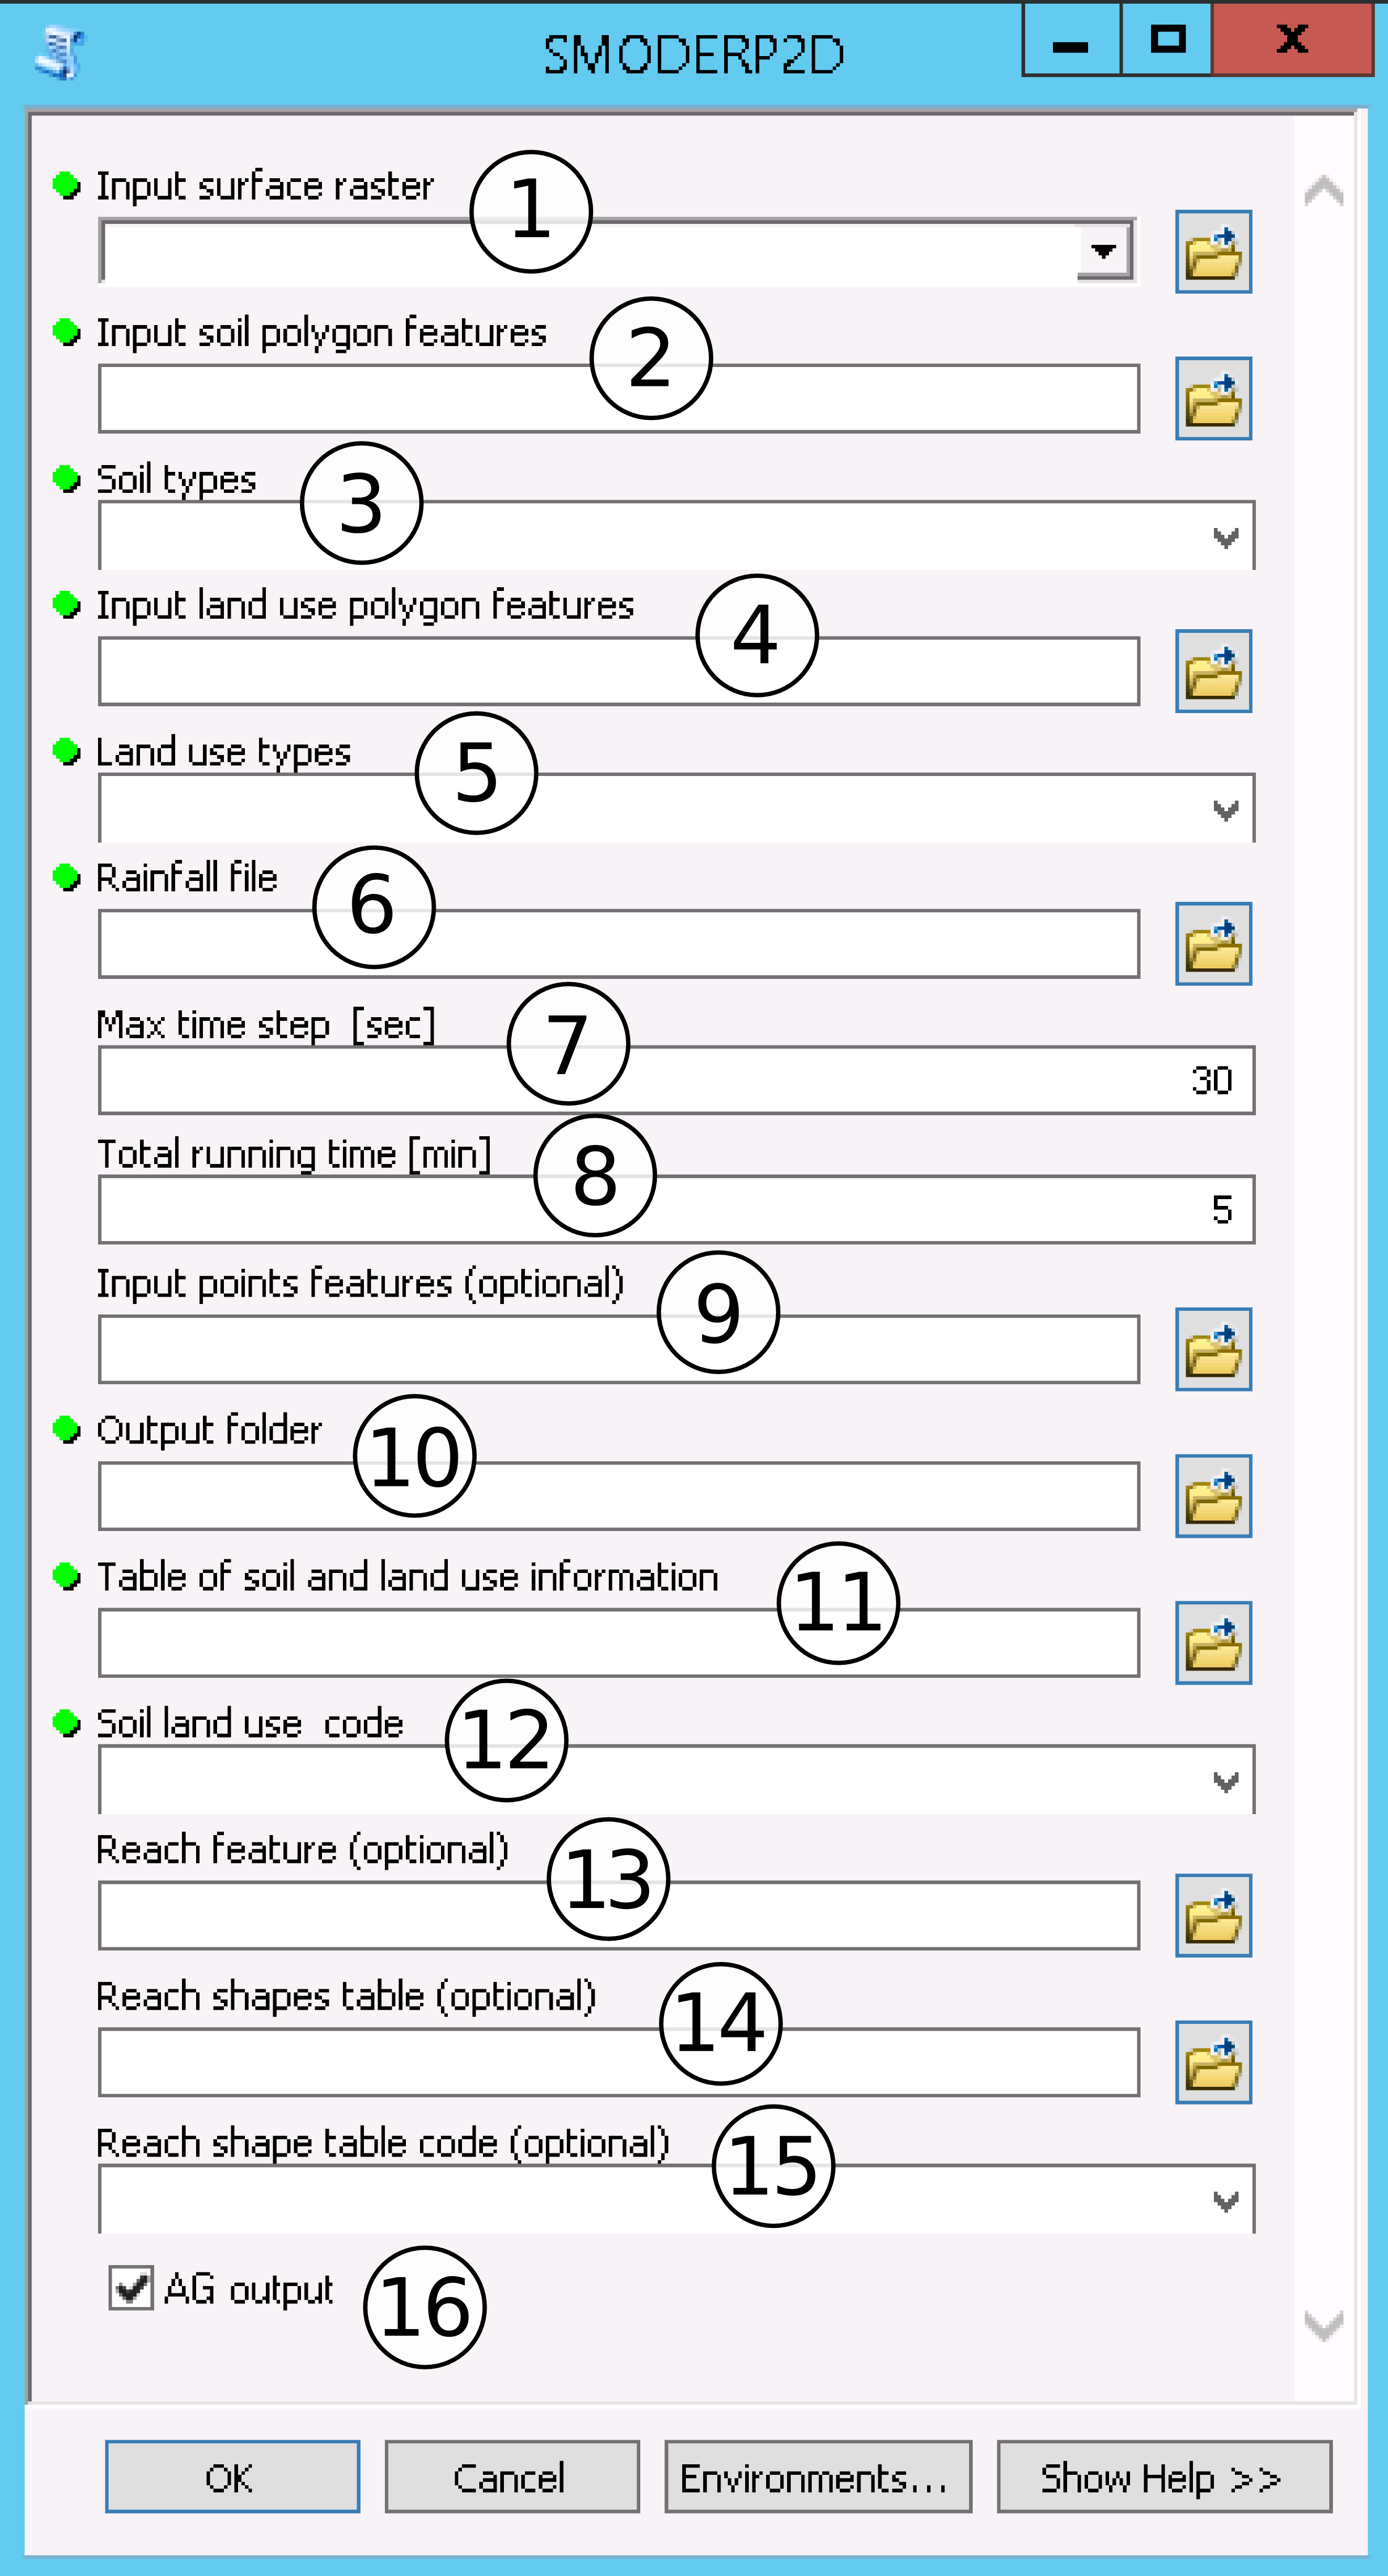
\includegraphics[width=\textwidth]{./img/toolboxpopis4.png}
    \end{minipage}\hfill
    \begin{minipage}[t]{.55\textwidth}
      \centering
      \vspace{0pt}
      {\scriptsize\sffamily
      \begin{tabular}{lp{.5\textwidth}l}
                     & Popis                                       & ArcGIS typ dat     \\
        \hline
	\circled{1}  & Cesta k digitálnímu modlu terénu            &  {\tt Raster layer} \\
	\circled{2}  & Cesta k vektorové vrstvě rozložení typu půd &  {\tt Shapefile} \\
	\circled{3}  & Název pole s id typů půd &  {\tt Field} \\
	\circled{4}  & Cesta k vektorové vrstvě využití území &  {\tt Shapefile} \\
	\circled{5}  & Název pole s id využití území &  {\tt Field} \\
	\circled{6}  & Cesta k souboru se srážkovými daty &  {\tt Text file} \\
	\circled{7}  & Maximální časový krok &  {\tt Double} \\
	\circled{8}  & Konečný čas výpočtu &  {\tt Double} \\
	\circled{9}  & Vrstva bodů pro výpis hydrogramů &  {\tt Shapefile} \\
	\circled{10} & Výstupní adresář &  {\tt Folder} \\
	\circled{11} & Tabulka s parametry modelu &  {\tt Table} \\
	\circled{12} & Označení pole v tabulce \circled{11} &  {\tt Field} \\
	\circled{13} & Cesta k vrstvě linií hydrografické sítě &  {\tt Feature Class} \\
	\circled{14} & Cesta k tabulce s geometrií úseků hydrografické sítě &  {\tt Table} \\
	\circled{15} & Název společného pole pro spojení \circled{13} a \circled{14} &  {\tt Field} \\
	\circled{16} & Volba formy výstupních souborů &  {\tt Boolean} \\
      \end{tabular}
      }
    \end{minipage}
    \caption{ArcGIS {\tt toolbox} a vysvětlenými parametry}
    \label{fig:toolbox}
  \end{figure}
%     \centering
%     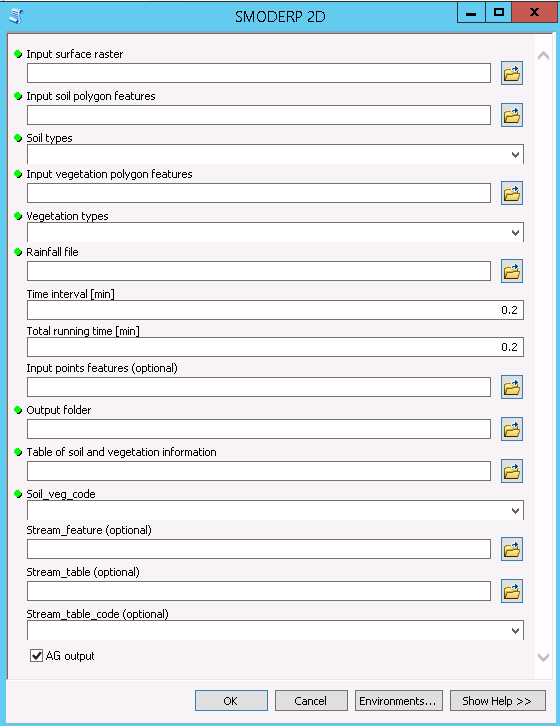
\includegraphics[width=0.75\textwidth]{./img/toolbox.png}
  
  
  
  
  
